\begin{abstract}
The day has come where the term "cloud" has become synonymous to the "internet" of 90's. Every major corporation is trying to find ways to scale their online services by squeezing in some sort of cloud technology into their core infrastructure while technology startups find the term "cloud" to be essential for attracting both new customers and investors. Among various aspects of cloud is its ability to easily scale various resources like computing (CPU), storage, networking, etc although mostly catered towards enterprise customers. 

Every internet user is exposed to some form of could service each day even when they are just checking their email or performing some web searches. Although it has been made possible to access multiple email accounts on an end-user's device using special email client applications, there has been little support to easily access the cloud storage associated with their email accounts. For example, even though a Gmail user is given access to gigabytes of free online cloud storage, there has been no easy or straightforward way to access this storage other then through Google's online Google Drive service. The situation is not very different for Microsoft Outlook service either. There also exists no open source software that can aggregate the multiple cloud storage accounts into one in an easy manner.

McFS project aims to develop a McFS (Multi-cloud File System) software framework using which users could access and/or combine their online cloud storage accounts in a seamless manner. The project also aims to prototype an online web portal which users could use to create required configurations for McFS clients running on their systems.
\end{abstract}


\section{Introduction}
In order to reduce the efforts required for the design and implementation of a basic McFS framework, I had decided to limit the scope of the project to the following runtime environment:

\begin{itemize}
  \item Support only Arch Linux and Ubuntu Linux 14.10 operating systems
  \item Requires Ruby MRI 2.1/2.2\cite{site:rubylang}
  \item Supports only Dropbox storage service
  \item Tested only on 64-bit Intel/AMD architecture
\end{itemize}

Although the software is being tested only on 64-bit Linux platform, since we do not depend on any hardware level interfaces, the software is expected to be readily portable to 32-bit Intel/AMD architecture. Portability across different Ruby implementations like JRuby, Rubinius, etc are not considered under the scope of this project although it is expected to be trivial. The reasons why I have chosen to support only Dropbox are mainly due to its large user base and availability of simple SDK for Ruby. Even though the project scope is limited to Dropbox, I have spent some time in analyzing feasibility of integrating with other services like Google Drive and will be briefly explained later. 

During initial investigation it was found that most of the cloud storage services do offer limited free storage for every user account which can easily be accessed using a REST (Representational State Transfer) based API with OAuth authentication. But in order to use OAuth authentication, we need to have an online web app (service) that can request access to user's cloud account. In order to accomplish this, I have also worked on setting up an online web portal (but tested only locally) at the domain bitmanor.net that can request this authentication.

\section{Main Objectives}
Following are the main objectives that have driven the project to its completion:
\begin{itemize}
	\item Implement the framework with modular design so that it can be easily extended to support new features and cloud storage services
	\item User should be able to easily add their Dropbox account(s) using a web portal using OAuth authentication mechanism
	\item User should be able to create a share (McFS share to be more specific) that would span across these accounts
	\item A Dropbox account should be sharable between multiple McFS shares
	\item Use local caching for better performance (if required and feasible)
	\item Implement the McFS Service which can expose its functionality as a REST API
\end{itemize}

\section{Software Architecture}
McFS Framework has been developed with modularity in mind and therefore has the following three major component types:

\begin{itemize}
	\item \textbf{service} is the core component that connects to all cloud storage services, creates shares that span across them and expose almost all the McFS core functionality as REST API.
	\item \textbf{views} can be thought of as a user interface for the functionalities provided by the McFS service.
	\item \textbf{synchronizers} are those that can synchronize configuration data among multiple McFS service instances running on separate machines.
\end{itemize}

More details about the component types are given below.

\begin{figure*}[t]
  \centering
  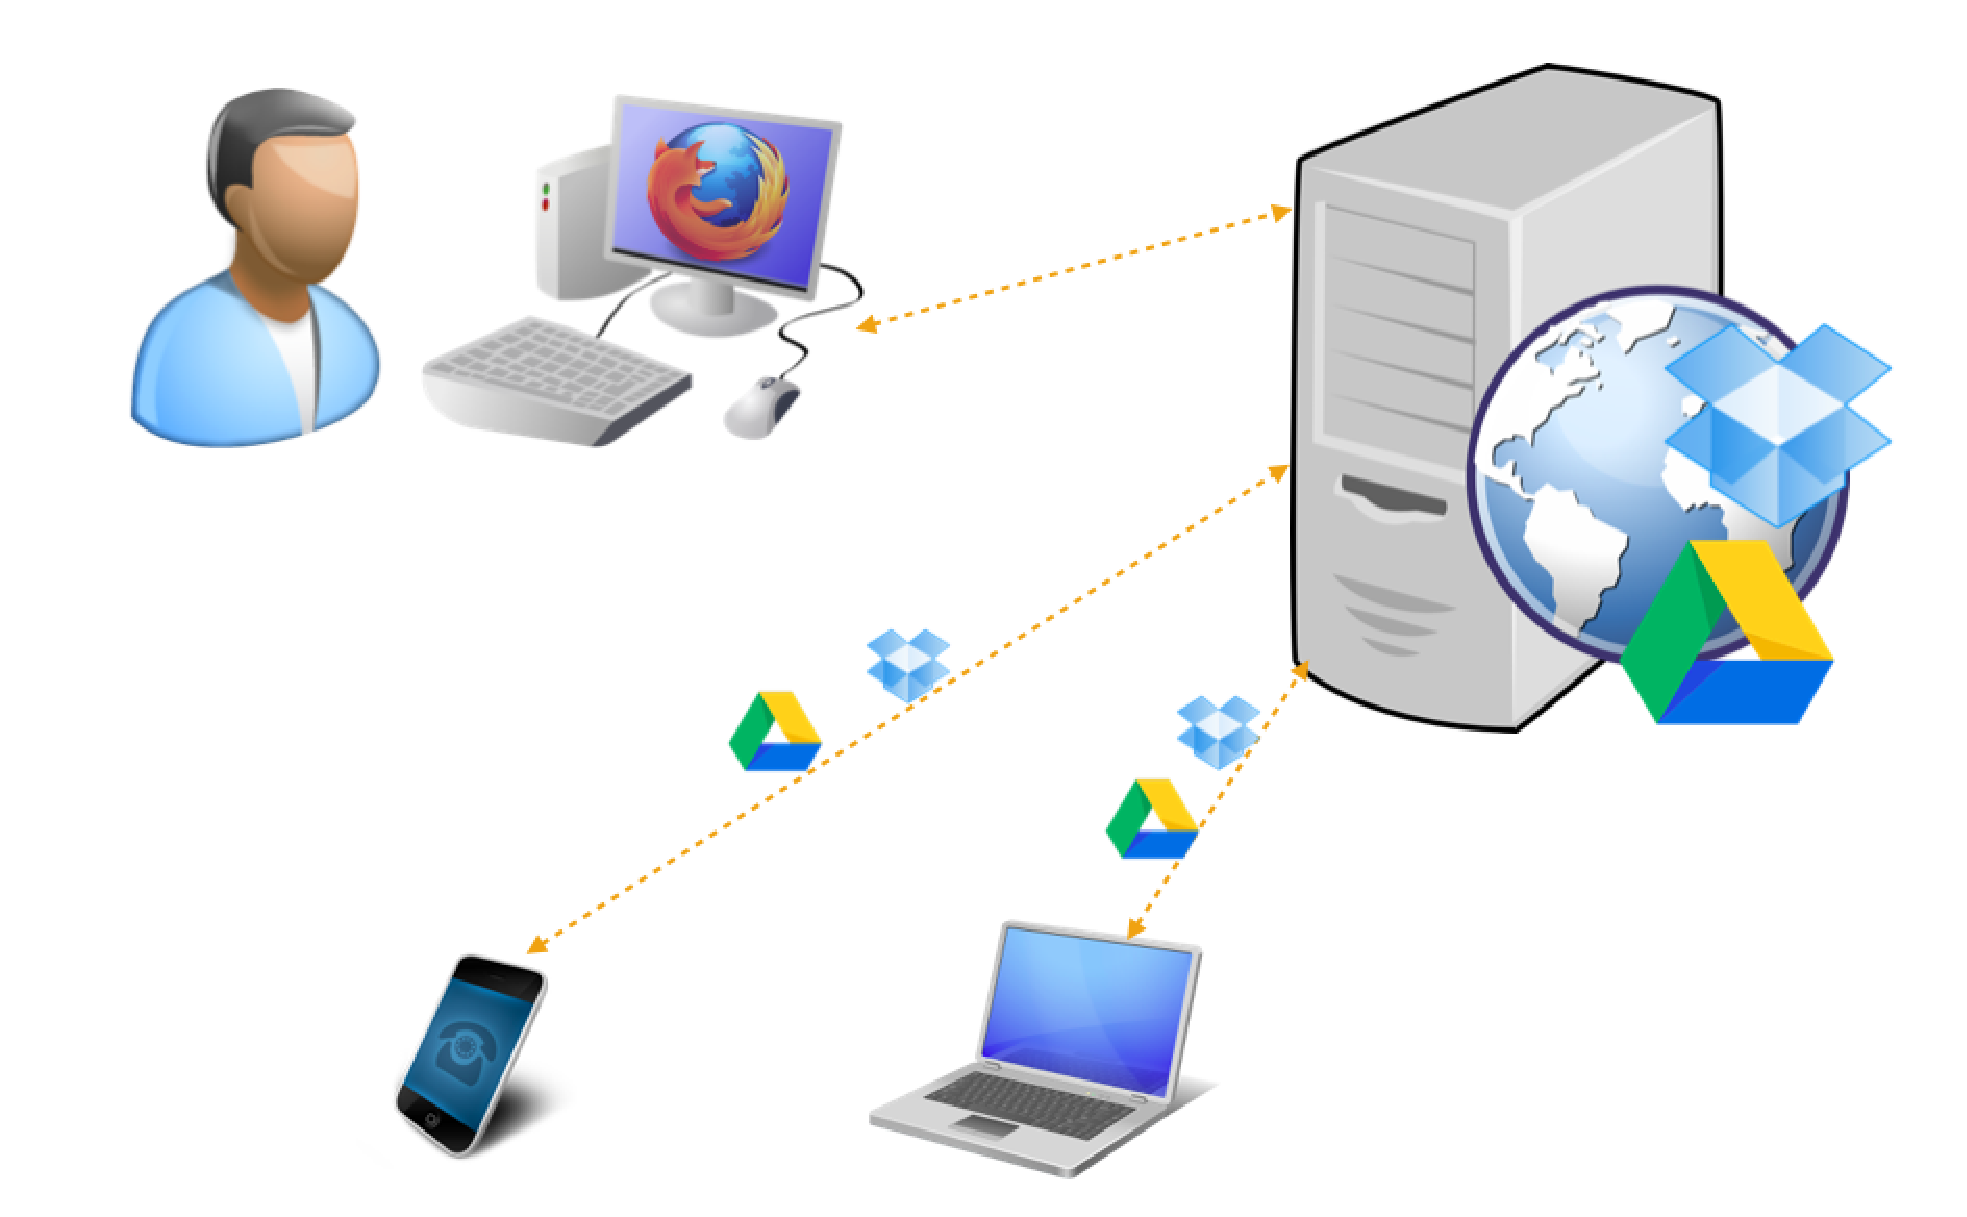
\includegraphics[width=0.8\textwidth]{usecase1}
  \caption{Typical Use Case}
\end{figure*}

\subsection{McFS Service}
The McFS Service is being developed using Ruby programming language and is designed to be published as a Ruby Gem\cite{site:rubygems}. The gem will be named as \textbf{mcfs-service} and can be installed using the gem command \textit{gem install mcfs-service} once the gem is published. The service when started on the system would start a web server within itself using which a REST API interface is exposed for external clients to interact with the service. The webserver is ran with a combination of Ruby Webmachine\cite{site:webmachineruby} and Celluloid Reel\cite{site:celluloidreel} frameworks in order to make it light weight and easy to implement and extend.

Following are the Ruby gems that are being used by the service:

\begin{itemize}
	\item \textbf{commander} gem provides easy command-line processing of the arguments provided to \textit{mcfs-service} application with automatic help menu generation.
	\item \textbf{dropbox-sdk} is the official gem provided by Dropbox for accessing and managing Dropbox accounts.
	\item \textbf{celluloid} gem provides an actor-based object concurrency framework that eases the parallelization of spanning requests to multiple cloud storage services.
	\item \textbf{reel} is a fast and light weight evented web server implemented on top of Celluloid framework.
	\item \textbf{webmachine} is a port of the Erlang Webmachine framework to Ruby that eases development of fault tolerant web services.
\end{itemize}

The project is hosted at https://github.com/mcfs/mcfs-service while more details about the McFS REST API is provided in a later section.

\subsection{McFS Views}
As mentioned before, \textit{views} are considered as user interfaces to the McFS Service that can be used to perform various actions which are:

\begin{itemize}
	\item Manage cloud storage accounts
	\item Manage McFS shares
	\item Manage McFS file systems (an McFS filesystem is a filesystem tree that can be accessed through REST API)
	\item Browse and modify contents of McFS file systems
\end{itemize}

Presently there are two views being developed actively:

\begin{itemize}
	\item \textbf{FUSE View} that can mount an McFS filesystem under a local directory using the Linux FUSE (Filesystem in Userspace)\cite{site:fuselinux} \cite{site:osxfuse} framework.
	\item \textbf{bitmanor.net} is an example web view which users could use to perform the actual OAuth authentication and thereby add cloud storage accounts to the service. The view also provides actions to create McFS shares and file systems.
\end{itemize}

The \emph{FUSE View} is being developed using Ruby and is planned to be published as \textbf{mcfs-view-fusefs} gem while the future plans for \emph{bitmanor.net} has not been made concrete. The FUSE View gem at present depends on the following third-party gems:

\begin{itemize}
	\item \textbf{rfusefs} enables implementation of file systems in userspace using the Linux FUSE api.
	\item \textbf{commander} for advanced command line option processing.
\end{itemize}

The FUSE View project is hosted at https://github.com/mcfs/mcfs-view-fusefs which can be referred for more details.

Since the very nature of the development of bitmanor.net is in a proprietary service oriented fashion, development of a separate generic web view is also under consideration. For now, I have registered the domain bitmanor.net with Google Domains with hosting on Linode while the site traffic is encrypted using SSL certificates. \emph{More details on the development of bitmanor.net can not be published at this point of time.}

\subsection{McFS Synchronizers}
McFS service does not initiate connections with other McFS services running over network as the service is expected to not act as a network client except for accessing third-party cloud storage services. Since bitmanor.net is a web view, we need to run a separate McFS Service on BitManor servers which processes the configuration actions requested by user using the website. Now when the user runs McFS service and FUSE View on his/her desktop, we need to somehow fetch the configuration data from bitmanor.net down to this service and that's where synchronizers come into play.

At present we have developed a synchronizer specific to bitmanor.net portal and named it mcfs-sycn-bitmanor which would also be the name of the Ruby gem when it becomes published. This open source project is hosted in Github under https://github.com/mcfs/mcfs-sync-bitmanor and performs the synchronization in a master-slave fashion where bitmanor.net and desktops act as master and slaves respectively.

\section{Use Case}

Figure 1 shows the typical use case that the framework aims to satisfy as part of this project. In this scenario, the user would first use his/her desktop to create a user account in bitmanor.net web portal. After this the McFS software framework that is installed on other computers and devices are connected (using synchronizer) to bitmanor.net using the same credentials that were used while creating bitmanor.net account.

The user can now use the web portal to create stores, shares and file systems which the synchronizers running on other systems would automatically fetch and update locally. Although the current synchronizer works in a master-slave fashion, I believe in future we would also be able to have a de-centralized one that does not require an online portal like BitManor.

\begin{figure*}
  \centering
  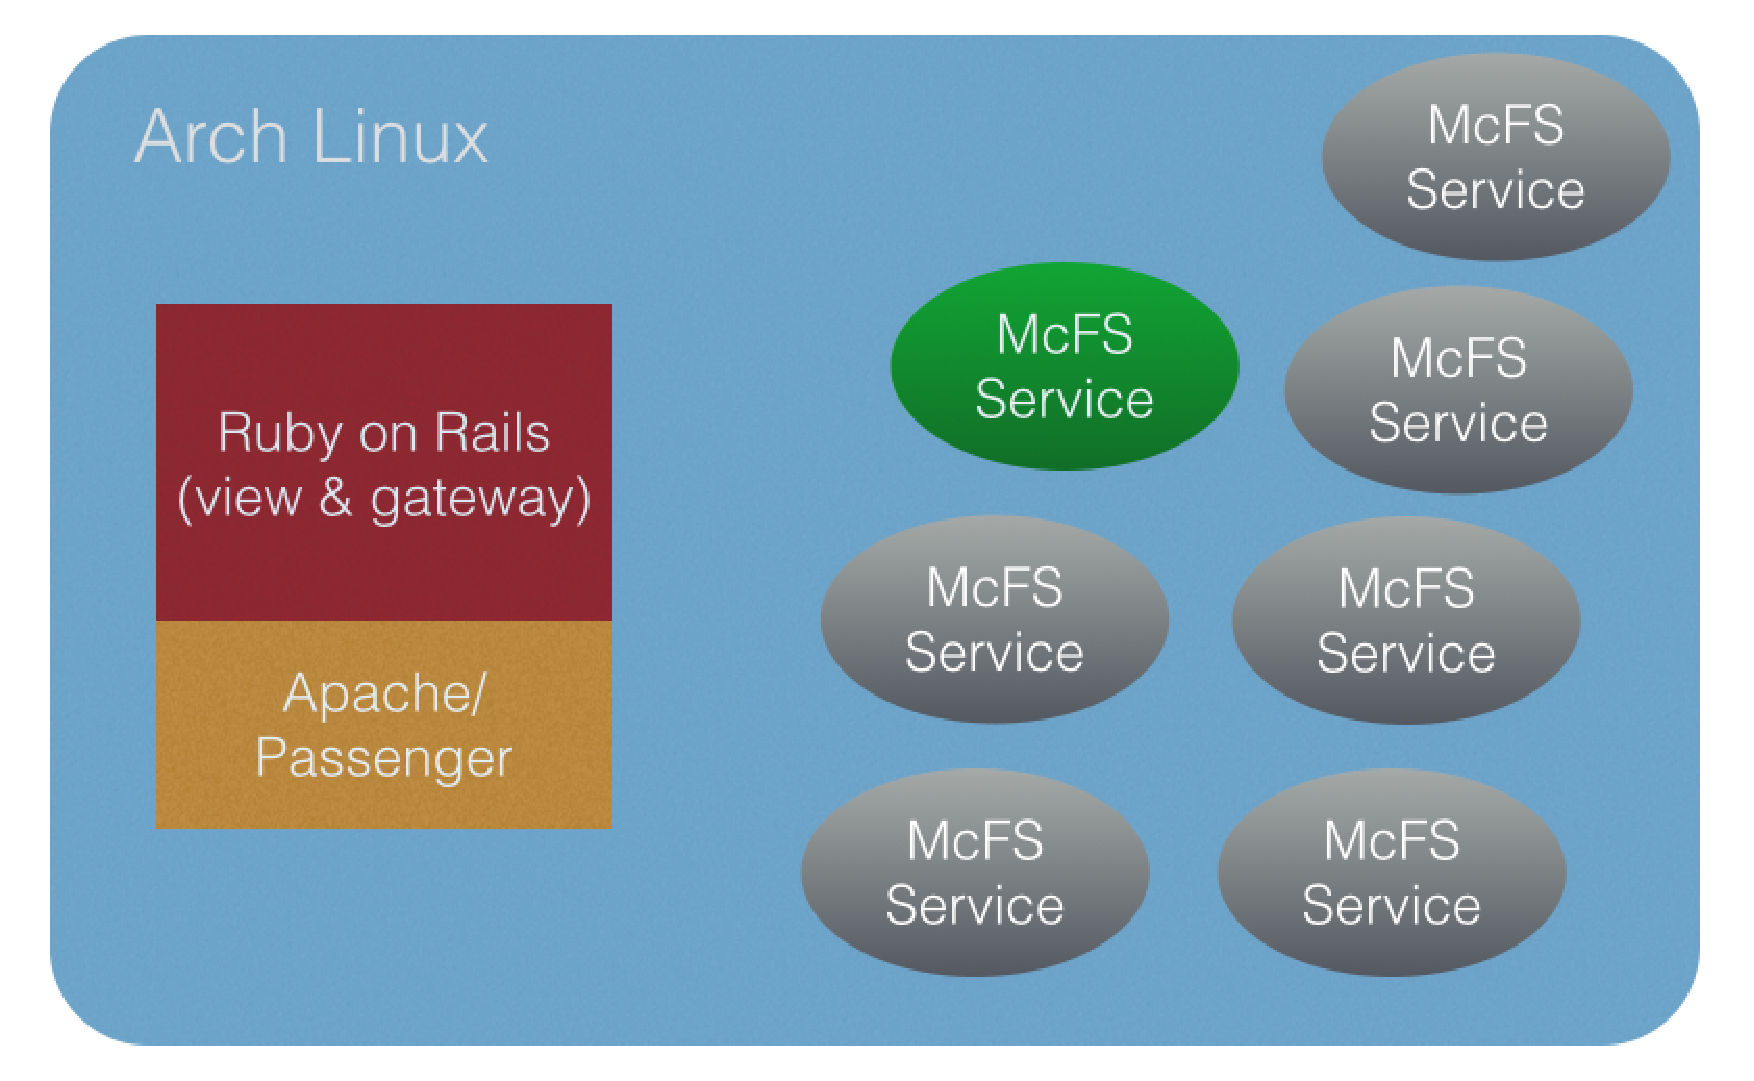
\includegraphics[width=0.8\textwidth]{server}
  \caption{McFS on Server}
\end{figure*}

\section{Stores, Shares and Filesystems}

In order to use McFS service, there are three important terminologies that need to be first understood by the user which are \emph{stores}, \emph{shares} and \emph{file systems}. Within the McFS service, all the three are considered to be a kind of \emph{namespace} where every name space is identified by a UUID (universally unique identifier).

\textbf{Stores} represent all kinds of data storage facilities available for the user. Generally we could divide this into local storage (hard drive connected to local system) and remote storage (eg. Dropbox, Google Drive, etc). At present, the framework support only Dropbox store which is also a remote store. Now, one of the issues with a remote store is the network latency for file operations which would make the usage of some views like the FUSE View, unbearable to end-user. In order to circumvent this, there is a metadata caching mechanism implemented generically for all remote stores.

\textbf{Shares} on the other hand are virtual name spaces that uses one or more stores to store the actual data. In the current implementation, we have only one type of share which is called McFSShare and it is used to combine multiple data stores to form a single namespace. All files written to an McFSShare is split into 64 kB chunks and distributed evenly across all stores. A directory named \emph{.McFS} is created under the root directory of all stores where a share-specific directory is created with the share UUID as the name. All files accessed within a share are routed to this directory, thereby avoiding any collision among multiple shares when they use the same data store.

\textbf{Filesystems} can be thought of as a Virtual Filesystem where we could mount any namespace that we wish to expose out of the service. An McFS file system acts as a gateway to client that want to access stores and shares. Use file management operations are allowed on file systems (and file systems only) by means of the REST API exposed by the service.

\emph{Please refer McFS Service REST API documentation for more information about various operations supported on the above namespace entities}.

\section {REST API}
As previously mentioned, all functionality of McFS Service is exposed through a REST API. There are specific end-points for managing stores, shares, and file systems. There is also an end-point to retrieve configuration updates from an McFS service which is presently used by the synchronizer to automatically update local McFS service with latest configuration from bitmanor.net portal.

All data exachange using this API uses YAML (YAML Ain't Markup Language) data exchange/serialization format. For detailed API documentation, please refer \emph{https://github.com/mcfs/mcfs-service/wiki/REST-API-v1}.

\section{Development}

\begin{figure*}
  \centering
  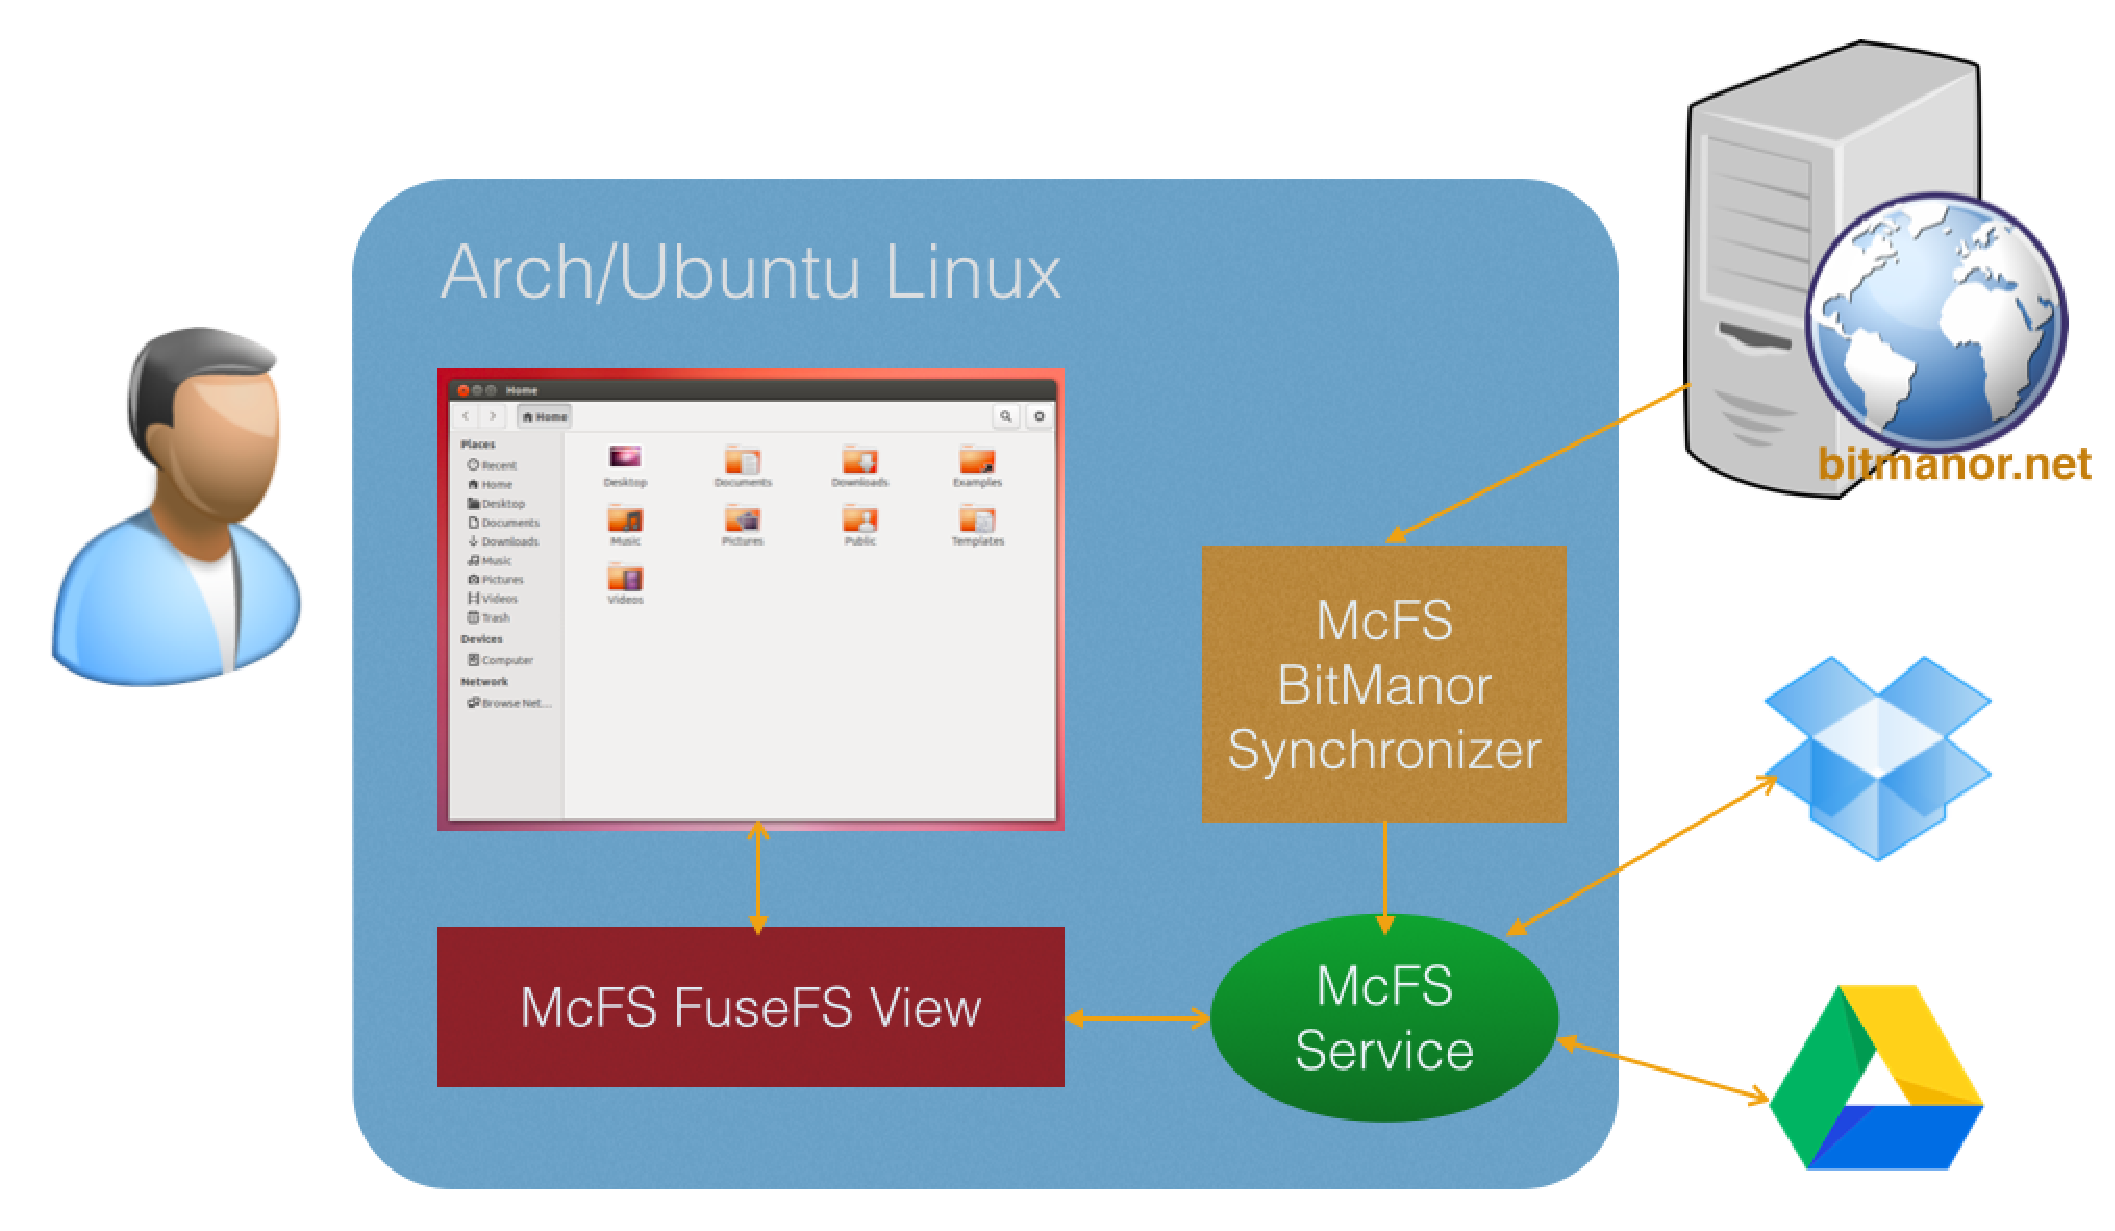
\includegraphics[width=0.8\textwidth]{client}
  \caption{McFS on Client}
\end{figure*}

All development and testing (including that of bitmanor.net website) were done one Arch Linux and Ubuntu Linux virtual machines that I have running on my Macbook Air under VirtualBox hypervisor. Figures 2 and 3 shows how a typical server or client machine would use the McFS framework components.

Typically on the web server, we would have just the McFS service running without any other views or synchronizers. The web site itself in this case would work as the required view for end-user. As of now, we expect the web server to run a separate instance of McFS Service process for each connected/logged-in user in order to provide better isolation and security. Executing separate instance of the service would also help us with scaling the service as the user base grows over time. Further analysis on computing, memory and networking resource requirements of McFS Service need to be investigated in order to properly quantify scalability requirements of the web service. In the case of bitmanor.net, we are hoping to run the website that was developed using Ruby on Rail on top of Apache web server with Phusion Passenger plugin.

On client side, we would run the same McFS service along with a synchronizer that would fetch configuration data periodically from the web server and update it in the local service. The FUSE View would be used to mount file systems created within the service on to a local directory. Once the directory is mounted, it can be accessed as any other directory within the local filesystem.

\emph{Note that when a store is initially added to a running server, its folder metadata is fetched and cached locally in order to enable fast browsing of directory contents mounted by the FUSE view}.

\subsection{Building}
Since Ruby is an interpreted programming language, there is no need to have the usual compile and link stages before running the modified software. Even then, some of the gems that we depend on (like rfuse) would require building its C extension components using a C compiler. This means that we need to ensure the compiler and make toolchain is installed on the development and test systems.

\subsection{Testing}
I constantly perform integration testing of the entire framework after implementation of each feature or fixing of bugs. Unit testing using RSpec is yet to be introduced although planned for a future date. A continuous integration service like Travis\cite{site:travisci} will be considered once the unit tests are worked on.

\subsection{Project Hosting}
All sub-projects of McFS framework will be hosted under the 'mcfs' Github organization account and the project home page will be accessible at http://mcfs.github.io.

\subsection{Release}
Releases for the software are to be made using Github portal. More details on this are not available at this time. Use of a Ruby packaging framework like \emph{Traveling Ruby}\cite{site:travelingruby} is also being considered.

\subsection{Portability}
At present, we aim the software to run correctly on the following platforms:

\begin{itemize}
	\item MRI \textgreater= 2.1 on Ubuntu Linux 14.10
	\item MRI \textgreater= 2.1 on Arch Linux (latest)
\end{itemize}

In future, we would like the software to run also on Rubinius and JRuby Ruby VMs with additional platform support for Mac OS and Windows (>= 7). In order to have FUSE View for OS X, we may have to add support for OSXFuse(https://osxfuse.github.io/). Similarly for Windows, we may have to look into the Dokan X (https://github.com/BenjaminKim/dokanx) framework.

\section{File Compression}
Transparent file compression of McFS shares are yet to be implemented. One of the difficulties we will face when it comes to compression is the calculation of file size during metadata operations. For example, when the user attempts to list the contents of a directory, the size of the file need to be determined separately from the size obtained from the store itself since the store has only the compressed file size. This means that the original file size need to be stored along with the file using some mechanism (ex. as part of file name itself).

Five algorithms that are being considered for file compression are Snappy, LZMA, BZ, GZ and Zip in order of their preference. Even though LZMA and Bzip are found to provide the best compression, Snappy, Zip and Gzip are light on CPU. We may need to come up with an algorithm to choose the compression format and level based on file type and access frequencies. For example, for least frequently (cold) used files, we could use Bzip or LZMA with highest compression level where as for most frequently used one, we could use snappy.

We also may have to adaptively choose the best compression algorithm among the same category by using some sort of heuristic mechanism. For example, when storing different parts of the same file (since the file is split), we could compress each part with a different compression format and find out the best format for the file. Once the best format is found for that file, later update could reformat the parts while making new writes.

This feature is not implemented since it's beyond the scope of this project.

\section{Local Caching}
When the user mounts an McFS account/share on the desktop, it would be best for performance to cache frequently and recently used data blocks in the local system itself. As of now we have only metadata level caching of a store's filesystem which currently helps in fast browsing of directory contents. This feature is not implemented since it's beyond the scope of this project.

\section{Service Tiering and Hot Data}
Service tiering and hot data migration are expected to be built on top of the framework at a future time. We hope to find a mechanism within the mcfs service to use heuristics to determine the performance of each connected account and use it to rank the accounts to partition them into different tiers. Hot data items which are determined by their access frequency can then be moved to a higher tier at an appropriate time. This feature is not implemented since it's beyond the scope of this project.
 
\section{Security and Privacy}
I take security and privacy very seriously. Apart from the HTTPS method used to access bitmanor online service, I intend to add the following security features in future to the framework:

\begin{itemize}
	\item Data stored as part of an McFS share are encrypted before being sent to a third-party data storage provider.
	\item Gems released as part of the project would be signed before release so that it can verified before installation.
\end{itemize}

\section{Chunk Size}
While spanning files across multiple storage, it need to be split into multiple chunks. Although the chunk size if presently kept as 64 KB, it would in future be made configurable or at least auto-determined for better overall latency and throughput.

\section{File Sharing}
A feature that is being requested by well wishers of the project is to be able to securely share files with their friends. This could mean a future need to integrate with social networking sites like Facebook, Twitter, Google+, etc. Since this feature require a lot of effort, it might be implemented only after the project submission.

This feature is not implemented since it's beyond the scope of this project.

\section{Advanced Technologies}
As I end this report, a few advanced technologies are also being investigated that could influence future progress of this framework.

Recently Google has come up with a new communication protocol which they call as QUIC (Quick UDP Internet Connections) that is aimed towards better latency and built-in security features. More details on this could be found at \emph{http://en.wikipedia.org/wiki/QUIC}.

There is also a plan to have the framework run in a de-centralized fashion by using peer-to-peer networking similar to that of Bit Torrent and Tor by utilizing technologies like Distributed Hash Table, NAT Traversal, etc.

\section*{Related Work}

\begin{itemize}
	\item SPANStor \cite{paper:spanstor} is a multi-cloud storage technology for cost-effective geo-replicated storage primarily meant for enterprises
	\item MultCloud \cite{site:multcloud} is an online web portal which can be used to access all the major online cloud storage accounts of a user
  \item Bittorrent Sync \cite{site:getsync} is a peer-to-peer file sharing proprietary application developed by Bittorrent, Inc.
\end{itemize}

\section{Coding Statistics}

Following are the approximate codelines implemented by me for various components in the McFS framework:

\begin{itemize}
	\item McFS Service - 2000
	\item McFS Fuse View - 300
	\item McFS Synchronizer for BitManor - 100
	\item BitManor web site - 400
	\item Miscellaneous - 100
\end{itemize}

\section{Test Setup}

Following steps are to be performed if someone require to use the McFS Service for testing with FUSE View:

\textbf{Step 1:} Download mcfs-service and mcfs-view-fusefs projects from Github using the URLs provided in previous sections

\textbf{Step 2:} Start the McFS service by changing into the mcfs-service directory and running \emph{ruby -Ilib bin/mcfs-service}. Before running the service, ensure you install all the necessary gems that the service depend on.
 
\textbf{Step 3:} If not already done so, follow instructions provided in \emph{https://www.dropbox.com/developers/core/start/ruby} to create your own Dropbox web app and authenticate it with a Dropbox account. Note down the authentication token.

\textbf{Step 4:} Use the \emph{/stores/add} REST API to add the new store with the token we obtained above. Use 'Dropbox' as the service name. You can use the uuidgen command line tool to generate a new UUID for the store.

\textbf{Step 5:} Use the \emph{/shares/add} REST API to add a new share (if required).

\textbf{Step 6:} Use the \emph{/filesystems/add} REST API to add a new filesystem which will be what we will use for mounting with FUSE View. Note down the filesystem UUID you give since it will be required while mounting the file system.

\textbf{Step 7:} Use the \emph{/filesystems/mountns} REST API to mount the stores and shares to the above created file system.

\textbf{Step 8:} On a different terminal, change to the mcfs-view-fusefs directory and run the view to mount the file system created above under a local directory. The command format is \emph{ruby -Ilib bin/mcfs-view-fusefs \textless filesystem uuid\textgreater \textless directory\textgreater }

Once the file system is mounted, you may use the terminal or file browser to browse through the contents and modify the files as required.

\emph{Please note that it may take a while for the store metadata to be cached in the service once the store is added. You are required to wait until the metadata caching is complete before doing further operation.}

\emph{It is also to be noted that the metadata cache is not updated further for changes in the remote store. But, any change made to the store though the local McFS service will be promptly updated within the local metadata cache.}


\section{Scalability and Performance}

\textbf{Scalability} is an important requirement when it comes to cloud related services and so does for McFS. As mentioned before, the service is spawned as a separate process listening on a different port for each logged in user on the web server. Scaling the service would be as easy as distributing these processes among other machines running within the data center. Within an McFS service, multiple stores and shares run concurrently as threads following the actor-based model provided by the Celluloid framework. This would help in parallelizing and load-balancing various McFS service requests. Although such is the case, we can not completely be sure about the limits of this until we test the service with enough cloud storage accounts. Multiple cloud accounts from Dropbox can not be used directly until we get production status for bitmanor.net web app which will require some time and effort.

As far as \textbf{performance} is concerned, we have a long way to go with analysis and optimizations. In present state, the software is heavily throttled due to various debug logs that we generate during runtime. Benchmarking by code profiling and request timestamping need to be done for further optimizations. For now, we have little or no overhead with file read operations when using shares or stores. But, write operations on the remote stores are found to take more than 5 times the time required to read. More of these can be determined by proper benchmarking and analysis.
